%%AMC:preprocess_command=prePythonTex4AMC
%%AMC:jobspecific=1
%%AMC:latex_engine=pdflatex --shell-escape

% Compilation Texmaker : Utilisateur/Commandes utilisateur
%--------------------------
% Shell Python :
% pdflatex --shell-escape -synctex=1 -interaction=nonstopmode %.tex|
% python /usr/share/texlive/texmf-dist/scripts/pythontex/pythontex.py %.tex|
% pdflatex --shell-escape -synctex=1 -interaction=nonstopmode %.tex|
%------------------------
% Copier-coller la ligne ci-dessous dans Utilisateur/Commandes Utilisateur/Editer Commandes Utilisateur
%------------------------
% pdflatex --shell-escape -synctex=1 -interaction=nonstopmode %.tex | python /usr/share/texlive/texmf-dist/scripts/pythontex/pythontex.py %.tex | pdflatex --shell-escape -synctex=1 -interaction=nonstopmode %.tex
%--------------------------

\documentclass[a4paper]{article}
\RequirePackage{etex}
\usepackage[utf8]{inputenc}    
\usepackage[T1]{fontenc}
\usepackage[french]{babel}
\selectlanguage{french} 
\usepackage[francais,bloc,completemulti]{automultiplechoice}    
\usepackage{fancyhdr,amssymb,amsmath}
%\usepackage{pgf,tikz}
\usepackage{tikz}
%\usepackage{pgfplots}
\usepackage{nopageno}
%\usepackage{fp}
%\pgfplotsset{compat=1.17}
\usetikzlibrary{arrows}
\usepackage{tabularx}

%\usepackage[onelanguage,french,linesnumbered,ruled]{algorithm2e}

% ---------- Utilisation de codes Python -----
\usepackage{pythontex}
\usepackage{csvsimple}
%----------------------------------------------
\def\barQ{b=1,m=-0.25}

\newif\ifpythontex
\newcommand{\includegraphicx}[2][]{%
\ifpythontex
\includegraphics[#1]{#2}
\fi
}
\pythontexfalse

\begin{pycode}
import numpy as np
import math
import random as ran
from fractions import Fraction as F
from sympy import *
from pylab import *


np.random.seed(12345)
sid=np.random.randint(1,999999999)
ran.seed(sid)
# IMPORTANT : Graine pour la fonction random


def genFonc(c):
    x=Symbol('x')
    fdev=F(1,2)*x**2-(c[0]+c[1])/2*x+c[0]*c[1]/2
    ffac=F(1,2)*(x-c[0])*(x-c[1])
    ffac2=(x-c[0])*(x-c[1])
    d=c[0]*c[1]/2-(c[0]+c[1])**2/8
    fcan=F(1,2)*(x-(c[0]+c[1])/2)**2+d
    s=(c[0]+c[1])/2
    fcan2=1/2*(x-s)**2+d
    fcan3=(x-c[1])**2+d
    return [latex(fdev),latex(ffac2),latex(fcan),latex(fcan2)]
    
def polyex21(b,c):
    x=Symbol('x')
    d=c-b**2
    f=F(1,2)*x**2+b*x+c
    return latex(f)
    
    
def polyex22(b,c):
    x=Symbol('x')
    d=c-b**2/2
    f=F(1,2)*(x+b)**2+d
    return latex(f)
    
def polyv2(b,p,d,q) :
	x=Symbol('x')
	myp = expand((x-b)**p*(x-d)**q)
	return latex(myp)

def polyv2(b,p,d,q) :
	x=Symbol('x')
	myp = expand((x-b)**p*(x-d)**q)
	return latex(myp)
	
def dp1x(a,b,c) :
    x=Symbol('x')
    y=Symbol('y')
    f=(a*y-1)/(b*x-1)**c

    g=diff(f,x,1)
    g2=g/b
    g3=g*(-1)
    g4=g2*(-1)

	 
    gl = latex(g)
    g2l = latex(g2)
    g3l = latex(g3)
    g4l = latex(g4)

    return np.array([gl,g2l,g3l,g4l])

def fonction(a,x1,x2) :
    x=Symbol('x')
    f=a*x*x-a*(x1+x2)*x+a*x1*x2
    fl=latex(f)
    d=np.random.randint(2,5)
    y=-a*(x1+x2)*x+a*(x1*x2+d**2)
    yl=latex(y)
    yi=a*(d**2+x1*x2-(x1+x2)*d)
    yib=a*(d**2+x1*x2+(x1+x2)*d)
    return np.array([fl,yl,d,yi,yib])

def canonique(a,b,c) :
    x=Symbol('x')
    delta=b*b-4*a*c
    xs=F(-b,2*a)
    ys=F(-delta,4*a)
    f=a*(x-xs)**2+ys
    fl = latex(f)
    f2=a*(x+xs)**2+ys
    f2l = latex(f2)
    f3=a*(x-xs)**2-ys
    f3l = latex(f3)
    f4=a*(x+xs)**2-ys
    f4l = latex(f4)
    return np.array([fl,f2l,f3l,f4l])

def sommet(a,b,c) :
    delta=b*b-4*a*c
    xs=F(b+c,2)
    ys=F(a*(xs-b)*(xs-c),1)
    return np.array([xs,ys])

def factor(b,c) :
    x=Symbol('x')
    ff=(x-b)*(x-c)
    ffl = latex(ff)
    ff2=(x-b)*(x+c)
    ff2l=latex(ff2)
    ff3=(x+b)*(x-c)
    ff3l=latex(ff3)
    ff4=(x+b)*(x+c)
    ff4l=latex(ff4)
    return np.array([ffl,ff2l,ff3l,ff4l])

def coeff() :
    pair=[2,4,6,8,10]
    impair=[1,3,5,7,9]
    a=np.random.randint(-7,7)
    while a == 0:
	    a=np.random.randint(-7,7)
    x1=np.random.randint(-10,-2)
    if (x1&1) :
    	x2=np.random.choice(impair) 
    else :
	    x2=np.random.choice(pair)
    if x2==-x1:
        x2=x2+2
    if -x1 > x2:
	    x3=x2
	    x4=-x1
    else:
	    x3=-x1
	    x4=x2
    return np.array([a,x1,x2,x3,x4])

def image(a,b,c,x) :
    return a*x*x+b*x+c

def signe(a):
    if a > 0:
        return ("positif","negatif")
    return ("negatif","positif")

def position(a):
    if a > 0:
        return ("au-dessous","au-dessus")
    return ("au-dessus","au-dessous")

def algosuite(u0,r,q,n):
    u=u0
    for i in range(1,n):
        u=q*u
        u=u+r
    return u

def wave():
    figure(figsize=(4,3))
    x = linspace(0, 4, 1001)
    plot(x, 2*sin(2*pi*x/4))
    xlabel('$x$ (m)')
    ylabel('$y$ (m)')
    grid(True)
   #name="wave"+id+".pdf"
    savefig('wave.pdf', bbox_inches='tight')
    return 1

def get_ant(dict_ai,img):
    return [k for k,v in dict_ai.items() if v == img]

def printSol(liste):
    sol="S=\{"+str(float(liste[0]))
    solf1="S=\{"+str(float(liste[0])-0.25)
    solf2="S=\{"+str(float(liste[0])+0.25)
    solf3="S=\{"+str(float(liste[0])-0.5)
    solf5="S=\{"+str(-1*float(liste[0]))
    
    if len(liste) == 1:
        solf4="S=\{"+str(float(liste[0])-1)
        solf6="S=\{"+str(-1*float(liste[0])+1)
    else:
        solf4="S=\{"+str(float(liste[0]))
        solf6="S=\{"+str(-1*float(liste[0]))

    for i in range(1,len(liste)):
        sol=sol+","+str(float(liste[i]))
        solf1=solf1+","+str(float(liste[i])-0.25)
        solf2=solf2+","+str(float(liste[i])+0.25)
        solf3=solf3+","+str(float(liste[i])-0.5)
        solf4=solf4+","+str(-1*float(liste[i]))
        solf5=solf5+","+str(float(liste[i]))
        solf6=solf6+","+str(-1*float(liste[i]))

    sol=sol+"\}"
    solf1=solf1+"\}"
    solf2=solf2+"\}"
    solf3=solf3+"\}"
    solf4=solf4+"\}"
    solf5=solf5+"\}"
    solf6=solf6+"\}"

    return [sol,solf1,solf2,solf3,solf4,solf5,solf6]
    

\end{pycode}







\element{test}{
\begin{questionmult}{test}\bareme{\barQ}
Test

\begin{reponseshoriz}
				\bonne{$U_{n}=\py{x1}n$}
				\bonne{$U_{n+1}=\dfrac{\py{x2}}{n}$} 				
 				\mauvaise{$U_{n+1}=U_{n}+n$}
 				\mauvaise{$U_{n+1}=U_{n}+1$}
			\end{reponseshoriz}
\end{questionmult}
}

\element{qqs}{
\begin{questionmult}{recurrence}\bareme{\barQ}
\AMCnoCompleteMulti
Parmi les relations suvantes, lesquelles sont de nature explicite~?
			\begin{reponseshoriz}
				\bonne{$U_{n}=\py{x1}n$}
				\bonne{$U_{n+1}=\dfrac{\py{x2}}{n}$} 				
 				\mauvaise{$U_{n+1}=U_{n}+n$}
 				\mauvaise{$U_{n+1}=U_{n}+1$}
			\end{reponseshoriz}
\end{questionmult}
}

\element{qqs}{
\begin{question}{explicite}\bareme{\barQ}
Parmi les relations suvantes, laquelle est exprimée par récurrence~?
			\begin{reponseshoriz}
				\mauvaise{$U_{n}=\py{x1}n$}
				\mauvaise{$U_{n+1}=\dfrac{\py{x2}}{n}$} 				
 				\mauvaise{$U_{n+1}=U_{0}+n$}
				\bonne{$U_{n+1}=U_{n}+\dfrac{1}{\py{x1}}$}
			\end{reponseshoriz}
\end{question}
}

\element{qqs}{
\pyc{q=np.random.randint(1,250)}
\begin{question}{recurrence2}\bareme{\barQ}
On considère une suite $(U_{n})$ telle que $U_{0}=8$ et chaque terme d’indice $n\ge 1$ vaut $\py{q}\%$ du précédent.
Une relation de récurrence pour la suite $(U_{n})$ est $U_{0}=8$ et:
\pyc{r=q/100}

			\begin{reponseshoriz}
				\bonne   {$U_{n+1}=\py{r}\times U_{n}$}
				\mauvaise{$U_{n+1}=\py{1+r}\times U_{n}$}
                                \mauvaise{$U_{n+1}=\py{r}n$}
                                \mauvaise{$U_{n}=\py{r}\times U_{n}$}
				\mauvaise{$U_{n}=\py{q}n$}
				\mauvaise{$U_{n+1}=\py{q}\times U_{n}$}
			\end{reponseshoriz}
\end{question}
}

\element{qqs}{
\begin{question}{sommerec}\bareme{\barQ}
\pyc{u0=np.random.randint(-9,-5)}
\pyc{u1=np.random.randint(-4,-1)}
On considère une suite $(U_{n})$ telle qu $U_{0}=\py{u0}$, $U_{1}=\py{u1}$ et chaque terme d’indice $n\ge 2$ vaut la somme des deux précédents.
Une relation générale de récurrence pour la suite $(U_{n})$ est:

			\begin{reponseshoriz}
				\bonne   {$U_{n+2}=U_{n}+U_{n+1}$}
				\mauvaise{$U_{n+1}=\py{u0}\times U_{n}\py{u1}n$}
                                \mauvaise{$U_{n}=U_{0}+U_{1}$}
                                \mauvaise{$U_{2}=U_{0}+U_{1}$}
			\end{reponseshoriz}
\end{question}
}




%--------
% DOCUMENT
%--------
\begin{document}

\newcommand{\sujet}{
\exemplaire{1}{
%\pyc{a=np.random.randint(2,7)} %

%\pyc{x1=np.random.randint(-6,-1)} %
 
%\pyc{x2=np.random.randint(2,8)} % 
\pyc{coefs=coeff()}
\pyc{a=coefs[0]}
\pyc{x1=coefs[1]}
\pyc{x2=coefs[2]}
\pyc{x3=coefs[3]}
\pyc{x4=coefs[4]}

\AMCassociation{\id}
%%% debut de l'en-tête des copies :

\begin{minipage}{.4\linewidth}
\centering\large\bf DS3 Mathématiques\\Vendredi 20.11.2020 \end{minipage}
\champnom{\fbox{    
                \begin{minipage}{.5\linewidth}
                  \begin{center} \nom{} \prenom{} \end{center}

                \end{minipage}
         }}


	%%% codage des numéros d'étudiants sur 3 chiffres par les candidats et encadré d'écriture manuelle des noms
	%\vspace*{3mm}
	%{\setlength{\parindent}{0pt}\AMCcodeGridInt{etu}{3}\hspace*{\fill}
	%\begin{minipage}[b]{12.8cm} %12cm

%----------------------------------------

	 %\hfill\champnom{\fbox{
	 %\begin{minipage}{0.96\linewidth}
	%	\vspace*{3mm} %3mm
		
	%	$\leftarrow$ {\footnotesize  Codez votre QCM-Number.\hspace{1.6ex}} || NOM :
		
	%	{\footnotesize  ( centaines, dizaines et unités )\hspace{2.19ex}} || Prénom :
		
	%	{\footnotesize  Complétez le cadre ci-contre} $\rightarrow$ \hspace{0.2ex} || Groupe :		
		%\hspace{4.438cm}|| Groupe :
	%	\vspace*{3mm}
	 %\end{minipage}
	  %  }
	  % }
	%\hfill  %\vspace{0.25ex}
%-------------------------------------

\begin{minipage}{0.96\linewidth}
\vspace*{3mm} %3mm
% texte de presentation 
%TEST125;Jean125;125 ## TEST102;Pierre102;102 TEST114;Marie114;114 ##TEST269;Helen269;269
\begin{center}\em  %\bf {center}

Les questions ont une unique bonne réponse. L'indiquer sur cette feuille en noircissant la case correspondante au stylo à bille noir. Aucune justification n'est demandée.
Les réponses fausses retirent un quart des points. Une absence de réponse n'enlève pas de points.
Pour rectifier une erreur, utilisez un correcteur "blanc" pour faire disparaître complètement la case noircie par erreur.	Calculatrice autorisée.
 

\end{center}

	\end{minipage}\hspace*{\fill}
	
	
\vspace{1ex}

%%% fin de l'en-tête



%\melangegroupe{qqs}
%\restituegroupe{test}

%Identifiant: \id
%\pyc{wave()}

%\includegraphicx[scale=0.4]{wave.pdf}

\begin{center}
\hrule\vspace{2mm}
\bf\Large Exercice 1
\vspace{2mm}\hrule
\end{center}

Soit la fonction f définie par la courbe représentative $C_{f}$ suivante:
\begin{center}
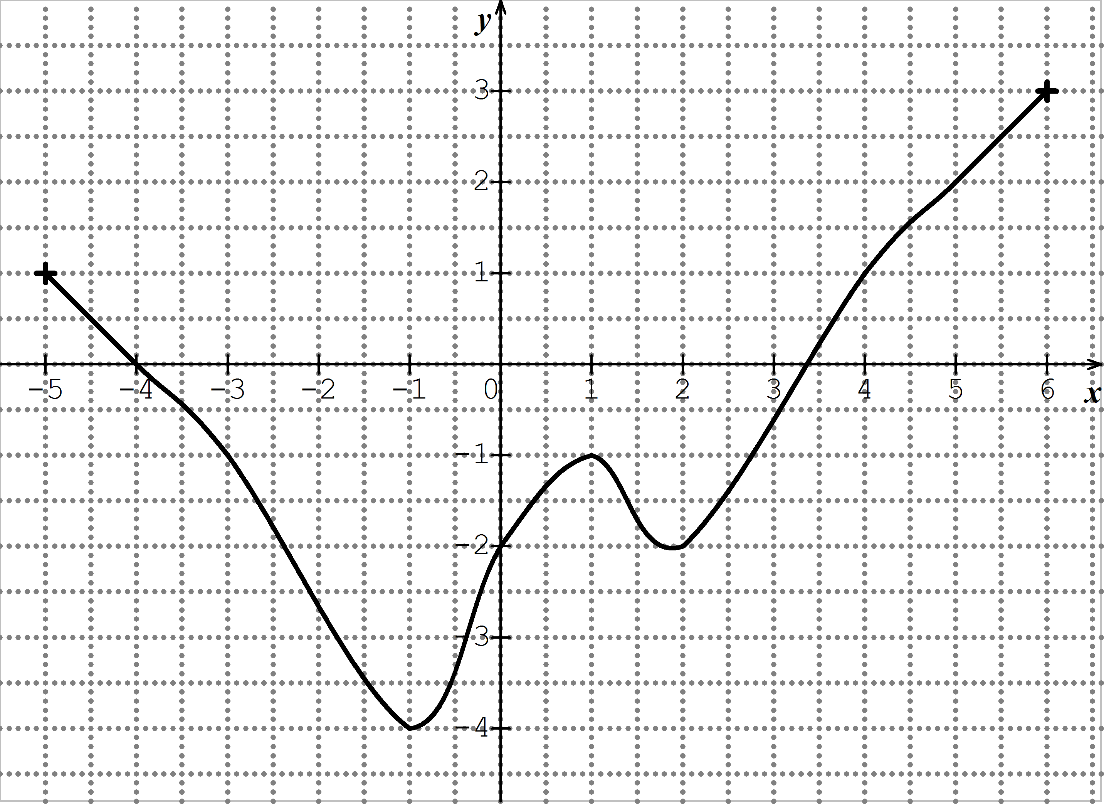
\includegraphics[scale=1]{data/graph1.png}
\end{center}

\begin{question}{domaineF}\bareme{\barQ}
Quel est le domaine de définition de $f$ ?
			\begin{reponseshoriz}
				\mauvaise{$[-6;6]$}
				\mauvaise{$[-5;7]$}
				\mauvaise{$[-4;1]$}
				\mauvaise{$[-4;3]$}
				\mauvaise{$[-5.5;6.5]$}
 				\mauvaise{$[-6;7]$}
				\bonne{$[-5;6]$}
			\end{reponseshoriz}
\end{question}

\pyc{sid=np.random.randint(1,999999999)}

\pyc{dict_ai={"-5":"1","-4.5":"0.5","-4":"0","-3.5":"-0.5","-3":"-1","-1.5":"-3.5","0":"-2","1":"-1","4":"1","5":"2","5.5":"2.5","6":"3"}}
\pyc{antecedents=["-5","-4.5","-4","-3.5","-3","-1.5","0","1","4","5","5.5","6"]}
\pyc{ran.seed(sid);ant_list=ran.sample(antecedents,3)}

\pyc{dict_ia={"-4":["-1"],"-3.5":["-1.5","-0.5"],"-1":["-3","1","2.75"],"0":["-4","3.4"],"1":["-5","4"],"1.5":["4.5"],"2":["5"],"2.5":["5.5"],"3":["6"]}}
%\pyc{images="-4","-3.5","-0.5","-3.5","-2","-1","2","2.5","3"}
\pyc{ran.seed(sid);img_list=ran.sample(list(dict_ia),4)}

\pyc{sym_list=["<","<=",">",">="]}
\pyc{ran.seed(sid);sym1=ran.choice(sym_list)}


\begin{question}{image0}\bareme{\barQ}
Déterminer graphiquement l’image de $\py{ant_list[0]}$ par la fonction $f$.
\pyc{ok=float(dict_ai[ant_list[0]])}
\pyc{f1=ok-0.5}
\pyc{f2=ok+0.5}
\pyc{f3=ok-1}
\pyc{f4=ok+1}



			\begin{reponseshoriz}
				\mauvaise{$\py{f1}$}
				\mauvaise{$\py{f2}$}
				\mauvaise{$\py{f3}$}
				\mauvaise{$\py{f4}$}
%				\mauvaise{$\py{sols[0]}}
				\bonne{$\py{ok}$}
			\end{reponseshoriz}
\end{question}

\begin{question}{image1}\bareme{\barQ}
Déterminer graphiquement l’image de $\py{ant_list[1]}$ par la fonction $f$.
\pyc{ok=float(dict_ai[ant_list[1]])}
\pyc{f1=ok-0.5}
\pyc{f2=ok+0.5}
\pyc{f3=ok-1}
\pyc{f4=ok+1}
			\begin{reponseshoriz}
				\mauvaise{$\py{f1}$}
				\mauvaise{$\py{f2}$}
				\mauvaise{$\py{f3}$}
				\mauvaise{$\py{f4}$}
				\bonne{$\py{ok}$}
			\end{reponseshoriz}
\end{question}

\begin{question}{image2}\bareme{\barQ}
Donner $f(\py{ant_list[2]})$
\pyc{ok=float(dict_ai[ant_list[2]])}
\pyc{f1=ok-0.5}
\pyc{f2=ok+0.5}
\pyc{f3=ok-1}
\pyc{f4=ok+1}
			\begin{reponseshoriz}
				\mauvaise{$\py{f1}$}
				\mauvaise{$\py{f2}$}
				\mauvaise{$\py{f3}$}
				\mauvaise{$\py{f4}$}
				\bonne{$\py{ok}$}
			\end{reponseshoriz}
\end{question}



\begin{question}{antecedents0}\bareme{\barQ}
\pyc{img=img_list[0]}
\pyc{sols=printSol(dict_ia[img])}
Determiner le(s) antécédent(s) de $\py{img}$ par la fonction $f$.
			\begin{reponseshoriz}
				\mauvaise{$\py{sols[1]}$}
				\mauvaise{$\py{sols[2]}$}
				\mauvaise{$\py{sols[3]}$}
				\mauvaise{$\py{sols[4]}$}
				\mauvaise{$\py{sols[5]}$}
				\mauvaise{$\py{sols[6]}$}
				\bonne{$\py{sols[0]}$}
			\end{reponseshoriz}
\end{question}

\begin{question}{antecedents1}\bareme{\barQ}
\pyc{img=img_list[1]}
Determiner le(s) antécédent(s) de $\py{img}$ par la fonction $f$.
\pyc{sols=printSol(dict_ia[img])}
			\begin{reponseshoriz}
				\mauvaise{$\py{sols[1]}$}
				\mauvaise{$\py{sols[2]}$}
				\mauvaise{$\py{sols[3]}$}
				\mauvaise{$\py{sols[4]}$}
				\mauvaise{$\py{sols[5]}$}
				\mauvaise{$\py{sols[6]}$}
				\bonne{$\py{sols[0]}$}
			\end{reponseshoriz}
\end{question}


\begin{question}{antecedents2}\bareme{\barQ}
\pyc{img=img_list[2]}
\pyc{sols=printSol(dict_ia[img])}
Résoudre graphiquement l'équation $f(x)=\py{img}$.

			\begin{reponseshoriz}
				\mauvaise{$\py{sols[1]}$}
				\mauvaise{$\py{sols[2]}$}
				\mauvaise{$\py{sols[3]}$}
				\mauvaise{$\py{sols[4]}$}
				\mauvaise{$\py{sols[5]}$}
				\bonne{$\py{sols[0]}$}
			\end{reponseshoriz}
\end{question}


\begin{question}{inequation}
\pyc{img=img_list[3]}
Donner tous les nombres $x$ tels que $f(x)\py{sym1}\py{img}$
\AMCOpen{lines=2}{\wrongchoice[F]{f}\scoring{0}\wrongchoice[P]{p}\scoring{0.5}\correctchoice[J]{j}\scoring{1}}
\end{question}


\begin{center}
\hrule\vspace{2mm}
\bf\Large Exercice 2
\vspace{2mm}\hrule
\end{center}

\pyc{ran.seed(sid);c = ran.sample(range(2,10,2), 2)}
\pyc{ran.seed(sid);racines = ran.sample(range(1,10), 2)}
\pyc{fonc=genFonc(c)}

%On considère la fonction définie sur $\mathbb{R}$ par $f(x)=\dfrac{\py{c[2]}}{\py{c[3]}}x^2-\py{c[1]}x+\py{c[0]}$.
\pyc{f21=polyex21(c[1],c[0])}
%On considère la fonction définie sur $\mathbb{R}$ par $f(x)=\dfrac{1}{2}x^2-\py{c[1]}x+\py{c[0]}$.
On considère la fonction définie sur $\mathbb{R}$ par $f(x)=\py{fonc[0]}$.

\pyc{ran.seed(sid);x = ran.sample(list(range(-10,-1))+list(range(1,11)), 3)}

\begin{question}{ex2image0}\bareme{\barQ}
Calculer l'image de $\py{x[0]}$ et $\py{x[1]}$ par $f$.

\AMCOpen{lines=1}{\wrongchoice[F]{f}\scoring{0}\wrongchoice[P]{p}\scoring{0.5}\correctchoice[J]{j}\scoring{1}}
\end{question}

\begin{question}{ex2image1}\bareme{\barQ}
Calculer $f(\py{x[2]})$.

\AMCOpen{lines=1}{\wrongchoice[F]{f}\scoring{0}\wrongchoice[P]{p}\scoring{0.5}\correctchoice[J]{j}\scoring{1}}
\end{question}


\begin{question}{ex2ante0}\bareme{\barQ}
Déterminer le(s) antécédent(s) de $\py{c[0]}$ par la fonction $f$.

\AMCOpen{lines=2}{\wrongchoice[F]{f}\scoring{0}\wrongchoice[P]{p}\scoring{0.5}\correctchoice[J]{j}\scoring{1}}
\end{question}

\begin{question}{ex2ante1}\bareme{\barQ}
Déterminer le(s) antécédent(s) de $\py{c[1]}$ par la fonction $f$.

\AMCOpen{lines=2}{\wrongchoice[F]{f}\scoring{0}\wrongchoice[P]{p}\scoring{0.5}\correctchoice[J]{j}\scoring{1}}
\end{question}

%\pyc{d=c[0]-c[1]**2/2}
%\begin{question}{ex2dev1}\bareme{\barQ}
%\pyc{f22=polyex22(c[1],c[0])}
%Développer $\dfrac{1}{2}(x-\py{c[1]})^2+\py{d}$
%Développer $\py{fonc[3]}$

%\AMCOpen{lines=2}{\wrongchoice[F]{f}\scoring{0}\wrongchoice[P]{p}\scoring{0.5}\correctchoice[J]{j}\scoring{1}}
%\end{question}

\begin{question}{ex2dev2}\bareme{\barQ}
Développer $\dfrac{1}{2}\py{fonc[1]}$

\AMCOpen{lines=2}{\wrongchoice[F]{f}\scoring{0}\wrongchoice[P]{p}\scoring{0.5}\correctchoice[J]{j}\scoring{1}}
\end{question}


\begin{center}
\hrule\vspace{2mm}
\bf\Large Exercice 3
\vspace{2mm}\hrule
\end{center}

\pyc{ran.seed(sid);a = ran.choice(range(-3,1))}
\newcommand{\tabVal}{
\begin{tabularx}{\linewidth}{|*{13}{>{\centering \arraybackslash}X|}}\hline
\parbox[][1cm][c]{1cm}{\centering $x$}
& \py{a-0.5} & \py{a} & \py{a+0.5} & \py{a+1} & \py{a+1.5} & \py{a+2} & \py{a+2.5} & \py{a+3} & \py{a+3.5} & \py{a+4} & \py{a+4.5}\\\hline
%& -1,5 & -1 & -0,5 & 0 & 0,5 & 1 & 1,5 & 2 & 2,5 & 3 & 3,5\\\hline
\parbox[][1cm][c]{1cm}{\centering $f(x)$}
& 
& 
& 
& 
& 
& 
& 
&
& 
& 
&
\\\hline
\end{tabularx}
}

La fonction $f$ est définie sur l’intervalle $[\py{a-0.5};\py{a+4.5}]$ par $f(x)=x^2-2x+1$

\begin{question}{ex3tab}\bareme{\barQ}
Par le calcul ou à l'aide de la calculatrice, compléter le tableau de valeurs ci-dessous.



\AMCOpen{contentcommand=tabVal,framerule=0pt}{\wrongchoice[F]{f}\scoring{0}\wrongchoice[P]{p}\scoring{0.5}\correctchoice[J]{j}\scoring{1}}
\end{question}

\newcommand{\inclusionImage}{\centering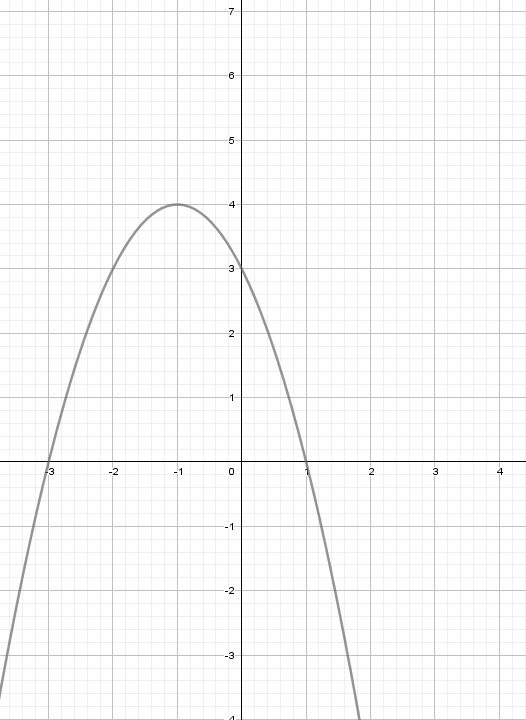
\includegraphics[scale=0.75]{data/graph2.jpg}\par}


\begin{question}{ex3graph}\bareme{\barQ}
Construire la courbe représentative de $f$ dans le repère ci-contre.
\begin{center}
\AMCOpen{contentcommand=inclusionImage,framerule=0pt}{\wrongchoice[F]{f}\scoring{0}\wrongchoice[P]{p}\scoring{0.5}\correctchoice[J]{j}\scoring{1}}
%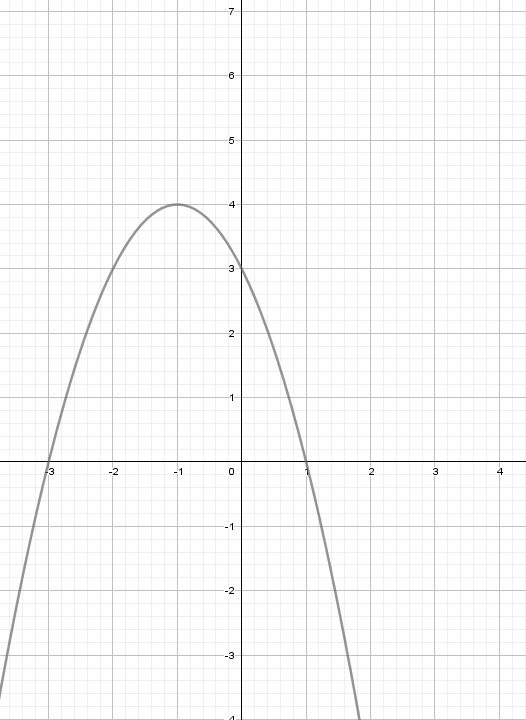
\includegraphics[scale=0.75]{data/graph2.jpg}
\end{center}
\end{question}

\pyc{val=ran.choice(range(-3,5,1))}
\pyc{sym2=ran.choice(sym_list)}
\begin{question}{ex3resgraph0}\bareme{\barQ}
Résoudre graphiquement $g(x)=\py{val}$
\begin{center}
\AMCOpen{lines=1,lineup=true}{\wrongchoice[F]{f}\scoring{0}\wrongchoice[P]{p}\scoring{0.5}\correctchoice[J]{j}\scoring{1}}
\end{center}
\end{question}

\pyc{sym2=ran.choice(sym_list)}
\begin{question}{ex3resgraph1}\bareme{\barQ}
Résoudre graphiquement $g(x)\py{sym2}f(x)$
\begin{center}
\AMCOpen{lines=1,lineup=true}{\wrongchoice[F]{f}\scoring{0}\wrongchoice[P]{p}\scoring{0.5}\correctchoice[J]{j}\scoring{1}}
\end{center}
\end{question}


\pyc{sym2=ran.choice(sym_list)}
\begin{question}{ex3resgraph2}\bareme{\barQ}
Résoudre graphiquement $g(x)\py{sym2}0$
\begin{center}
\AMCOpen{lines=1,lineup=true}{\wrongchoice[F]{f}\scoring{0}\wrongchoice[P]{p}\scoring{0.5}\correctchoice[J]{j}\scoring{1}}
\end{center}
\end{question}


%---------------
%--

}
}
\csvreader[head to column names]{../liste.csv}{}{\sujet}

\end{document}

